\chapter{\IfLanguageName{dutch}{Stand van zaken}{State of the art}}%
\label{ch:stand-van-zaken}

% Tip: Begin elk hoofdstuk met een paragraaf inleiding die beschrijft hoe
% dit hoofdstuk past binnen het geheel van de bachelorproef. Geef in het
% bijzonder aan wat de link is met het vorige en volgende hoofdstuk.

As previously mentioned, this research focuses on the cryptocurrency market and it's relation with social media sentiment. This chapter will start by introducing some of the key theories and concepts which provide essential context related to the chosen topic.
Furthermore we will be going over previous studies and provide a comprehensive summary of earlier research. Finally we will be explaining why our research is a valuable addition to the topic.
% Pas na deze inleidende paragraaf komt de eerste sectiehoofding.

%Dit hoofdstuk bevat je literatuurstudie. De inhoud gaat verder op de inleiding, maar zal het onderwerp van de bachelorproef *diepgaand* uitspitten. De bedoeling is dat de lezer na lezing van dit hoofdstuk helemaal op de hoogte is van de huidige stand van zaken (state-of-the-art) in het onderzoeksdomein. Iemand die niet vertrouwd is met het onderwerp, weet nu voldoende om de rest van het verhaal te kunnen volgen, zonder dat die er nog andere informatie moet over opzoeken \autocite{Pollefliet2011}.

%Je verwijst bij elke bewering die je doet, vakterm die je introduceert, enz.\ naar je bronnen. In \LaTeX{} kan dat met het commando \texttt{$\backslash${textcite\{\}}} of \texttt{$\backslash${autocite\{\}}}. Als argument van het commando geef je de ``sleutel'' van een ``record'' in een bibliografische databank in het Bib\LaTeX{}-formaat (een tekstbestand). Als je expliciet naar de auteur verwijst in de zin, gebruik je \texttt{$\backslash${}textcite\{\}}.
%Soms wil je de auteur niet expliciet vernoemen, dan gebruik je \texttt{$\backslash${}autocite\{\}}. In de volgende paragraaf een voorbeeld van elk.



\section{Cryptocurrencies }%
\label{introductie}
Over the years it has become increasingly difficult to form a general definition of cryptocurrencies, as the space has evolved rapidly and many new coins have emerged. However cryptocurrencies can be broadly defined as followed: \bigbreak
Cryptocurrencies are digital assets which use cryptography in order to secure transactions between users, to control the creation of additional units and to publicly monitor past transfers. A cryptocurrency represents an open source peer-to-peer network where users can interact and transact with each other, without the need of a 3rd party. In order to accomplish all of this, most of the cryptocurrencies make use of blockchain technology.~\autocite{Wolfgang2019} \bigbreak

\section{Blockchain technology and distributed ledgers }

There are many different types of blockchains, each with their own characteristics. All of them  fall under the broader category of ‘distributed ledgers’. A distributed ledger is a type of database which is geographically spread across different locations and is typically public. All of the records are stored one after the other and are verified by the parties involved. A distributed ledger is not in centralized control, so it generally requires more trust in the various validators or operators of the ledger. However, a benefit of a distributed ledger is that it operates without a single point-of-failure, unlike standard databases.~\autocite{Hancock2016} \bigbreak 

Typically distributed ledger technology is implemented by using a blockchain. As mentioned earlier, blockchains have their own rules and standards for how a ledger is created and maintained. They have different rules for participation, different network rules, different specifications on how to create transactions and different methods of storing data. But they usually contain the following concepts: 
\begin{enumerate}
\item	A data store which records changes in the data. Usually this is financial data but it could  be any kind of data. This data is stored in so-called ‘blocks’, which are linked together via cryptographic hashes, thus forming a chain.
\item	The data is replicated across a different number of independent systems. All the participants work together to ensure that the data remains correct and is visible to everyone.
\item	Peer-to-peer rather than a traditional client-server network architecture. There is no single centralized coordinator, instead the data is spread by all participants.
\item	In order to prove authenticity and ownership, the blockchain uses cryptographic methods such as digital signatures and hashes. ~\autocite{Lewis2018}
\end{enumerate} \bigbreak

\section{Smart contracts and decentralized finance}\bigbreak

Decentralized finance, commonly referred to as DeFi, is one of the most exciting new developments within the cryptocurrency space. DeFi consists of multiple protocols that replicate existing financial services in a more verifiable and transparent way, removing the need for centralized third party actors like banks or exchanges. These protocols are often referred to as DApps (Decentralized Applications), which are built on blockchains and use smart contracts for their app logic.~\autocite{Schaer2021}\bigbreak

Smart contracts are programmable scripts that automate the actions required in an agreement or contract. They are commonly used within DApps on a blockchain, in order to complete transactions between two parties. Once a transaction is executed by a smart contract, it is irreversible and transparent for everyone on the network to witness.~\autocite{Schaer2021}There are multiple smart contract programming languages, the most popular being Solidity which is used on the Ethereum blockchain~\autocite{Chirag2022}.\bigbreak

One example of a DApp using smart contract technology, would be Aave. This is an application which allows users to lend and borrow cryptocurrency assets between each other, without the need of a third party. Suppliers can deposit their funds in a smart contract and earn interest, while borrowers are able to borrows funds relative to their collateral. The smart contract is public, open source and audited by a third party in order to make it completely safe to lock up funds. The suppliers can withdraw their funds on demand, and the borrowers can repay their loan at any time~\autocite{Boado2020} As of writing this essay, a total of 7.5 billion dollar in value is locked into the Aave protocol~\autocite{Aave}.\bigbreak

These DApps have become increasingly popular over the last couple of years. Between April of 2020 and April 2022 the total amount of active users increased from 450,000 to 4.5 million~\autocite{Chen2022}. During the same time period, the total value locked in all of the decentralized applications combined went from around 500 million dollars to more than 230billion dollars~\autocite{Matsuoka2022}. \bigbreak 

\section{Investing in cryptocurrencies}

As this research is centered around the price of cryptocurrencies, it is important to answer some questions surrounding investment in cryptocurrencies. \bigbreak

\textbf{How do you invest in cryptocurrencies ?} \bigbreak

Cryptocurrencies trade on one or more exchanges, both prices and liquidity can differ between different exchanges.~\autocite{Lewis2018a} The first type of exchange is the centralized exchange which is controlled by a 3rd party. These act as a middle man between banks and investors, allowing people to deposit and withdraw traditional currencies from a personal bank account onto the exchange, and vice versa . Once an investor deposits traditional currency onto the exchange, they can then freely trade that currency for a cryptocurrency of choice.~\autocite{Reiff2021}\bigbreak

A second type of exchange is the decentralized exchange, commonly abbreviated as DEX, which is a peer-to-peer marketplace where users can freely trade with each other. The trades and transactions on a DEX are executed on the blockchain, which acts as a ledger and records all of the transactions. Although they are more in line with the decentralized nature of cryptocurrencies, DEX’s do not offer any way to connect to a standard bank account. Therefore every investor must always use a centralized exchange in order to fund their initial investment.
~\autocite{Aspris2021}\bigbreak

\textbf{What determines the value of a cryptocurrency ?} \bigbreak

The price of a cryptocurrency is completely determined by the market. The basic rules of supply and demand apply, if  the supply remains constant and demand increases then the price rises. If the demand drops then the reverse happens. It is up to the market participants to decide the fair value of a cryptocurrency.~\autocite{Lewis2018a} \bigbreak

Unlike more traditional investments like stocks, there is no inherent or fair value for a cryptocurrency. Although there are differing opinions on how to value the stock of a company, most of the investors agree that the correct value lies between a certain price range. This price range is based on multiple factors such as the company’s cash flow, earnings, dividends and growth rate.~\autocite{Schmidt2023} These methods of valuation are not applicable for a cryptocurrency, which also contributes to its volatility. \bigbreak

\textbf{What causes prices to change ?} \bigbreak

The buyers and sellers of cryptocurrencies are influenced by several different factors.
\begin{enumerate}
    \item 	Technical successes. For example when a cryptocurrency successfully implements a technical upgrade which makes it more useful or easier to use.~\autocite{Lewis2018a}
    \item	Government regulations. Because of their novelty, new regulations are still being established in order to control cryptocurrencies. These new laws can affect the potential of some assets. ~\autocite{Lewis2018a}
    \item	Adoption. As the ledger is publicly available, it is easily determined how many active users a certain cryptocurrency has. If the user population keeps on rising, traders then speculate the demand should follow. ~\autocite{Lewis2018a}
    \item	Celebrity endorsements. A lot of cryptocurrencies form partnerships with celebrities in order to legitimize themselves in the eyes of the public. Announcements of these partnerships can lead to short-term price movements.~\autocite{Lewis2018a} 
    \item	Macroeconomic conditions. Like all markets, the cryptocurrency market is closely tied to the broader economy. Inflation, interest rates and unemployment all have their effect on the price of assets.~\autocite{Bouronikos2022} 
    \item	Social media and general sentiment. News about cryptocurrencies and social media discussions can effect the general sentiment of traders. Most cryptocurrency investors are active on social media platforms such as Twitter, Reddit or Instagram, and admit that these platforms influence their investment choices.~\autocite{Lewis2018a} 
\end{enumerate}

\textbf{Why do people invest in cryptocurrencies? } \bigbreak

There a many different reasons why investors choose to invest in cryptocurrencies. According to a study in Asia, researchers found the following reasons to be most prominent:

\begin{enumerate}
    \item Short term profit seeking (42\%)
    \item To learn more about cryptocurrencies (34\%)
    \item A strong belief in the project and underlying technology (32\%)
    \item To diversify their overall investment portfolio (30\%)
    \item As a long term investment or retirement plan (29\%)~\autocite{OECD2019}
\end{enumerate} \bigbreak


In a different study researchers interviewed investors in order to find out what made them invest into cryptocurrencies for the first time. The research showed that a lot of people first got introduced to cryptocurrencies by a friend, or by social media. The interviewees reported they experienced a fear-of-missing-out as it seemed everyone around them made a lot of money in a short period of time. This made them want to invest as well, in order to chase short-term profits. Most of them saw investing in cryptocurrencies more as a gamble, than an actual investment. With participants of the study also mentioning they just invested for fun and that they wanted to know what all the hype was about. They were aware of the fact that the risk involved was very high, and knew that almost all of their starting capital could be lost.\autocite{Magnusson2022} \bigbreak

\section{Behavioral Economics} \bigbreak

The term of behavioral economics is used to describe the study of decision making and behavior of humans in an economic setting, it integrates behavioral science with economic principles. According to traditional economics like John Stuart Mill, humans will always act in the most rational way that fully maximizes their long-term gains. Individuals are assumed to have a complete and correct understanding of all the costs and benefits of the possible actions they can take.\autocite{Reed2013} \bigbreak

Behavioral economists do not agree with this notion and expect that people will often act in an irrational manner, making decisions that are not always optimal and in their own best interest. That even though there a clear optimal options, individuals are still susceptible to certain temptations and biases which cloud their judgement.\autocite{Reed2013} \bigbreak

One famous example of a behavioral economics theory is Prospect theory, developed by Amos Tversky and Daniel Kahneman in 1979. The theory was cited as one the reason’s to award Kahneman the 2002 Nobel Memorial Prize in Economics. It was one of the first studies that challenged the  assumption of human rationality within traditional economics.\autocite{Kahneman1979} \bigbreak

The study suggests that humans experience losses of capital in a different way than similar gains, which leads to irrational decision making when faced with certain scenarios. The study showed that people were more risk seeking in order to avoid losses, and more risk averse when seeking gains.\autocite{Kahneman1979} Consider the following two scenario’s:
\begin{enumerate}
    \item A 95\% chance to win \$10 000 dollars or a 100\% chance to win \$9 499
    \item 2.	A 95\% chance to lose \$10 000 dollars or 100\% chance to lose \$9 499  
\end{enumerate} \bigbreak

In the first scenario, people were more likely to choose the second option of a guaranteed gain. However in the second scenario, people were more risk seeking and preferred the first option that has a chance to avoid losses. The thought of a sure loss seemed too painful, and the hope of a complete relief too enticing. The study supported the idea that emotions do affect the decision making of humans and that they will not always act is the most rational way.\autocite{Kahneman2011} \bigbreak

\section{Behavioral Finance and Herd Behavior} \bigbreak

Behavioral finance is a subfield of Behavioral economics, which focuses more on the psychology of investors within financial markets.  Once again it assumes that market participants can often act in an irrational manner, as they are influenced by human emotion and suffer from certain cognitive limitations. These inefficient decisions can impact markets on a large scale and cause disruptions which lead to market anomalies. A market anomaly describes a market which is inefficient and inconsistent with standard theories of asset pricing. \autocite{Kapoor2017} \bigbreak

Herd Behavior is a general human behavior which can also influence decision-making within financial markets. Within the context of behavioral finance, herd behavior refers to the phenomenon where people group together and blindly follow what they believe other investors are doing.  Charging into investments without reflecting upon them individually and often without adequate knowledge.  This behavior can lead to increased volatility and the forming of market bubbles, as big groups of market participants all choose to buy or sell at the time.\autocite{Bikchandani2000} \bigbreak 

One famous example of this behavior relates to the dotcom bubble of late 1990’s. During the 1990’s the Internet started to gain traction worldwide, and people began to have easy access to the World Wide Web through web browsers. Investors became very eager to invest in this new technology, and did so without properly evaluating the correct valuation of Internet-related companies.\autocite{Morris2008} During this time, the media also continually covered the topic in a positive way, leading to even more people investing without doing much research. This irrational optimism and ignorance lead to a market bubble where the companies within the sector became severely overvalued.\autocite{Sanjana2018} The bubble then finally burst in the early 2000’s, with multiple companies going bankrupt and the entire sector losing more than 75\% of it’s stock market value. \autocite{CFI2023} \bigbreak

\begin{figure} [h]
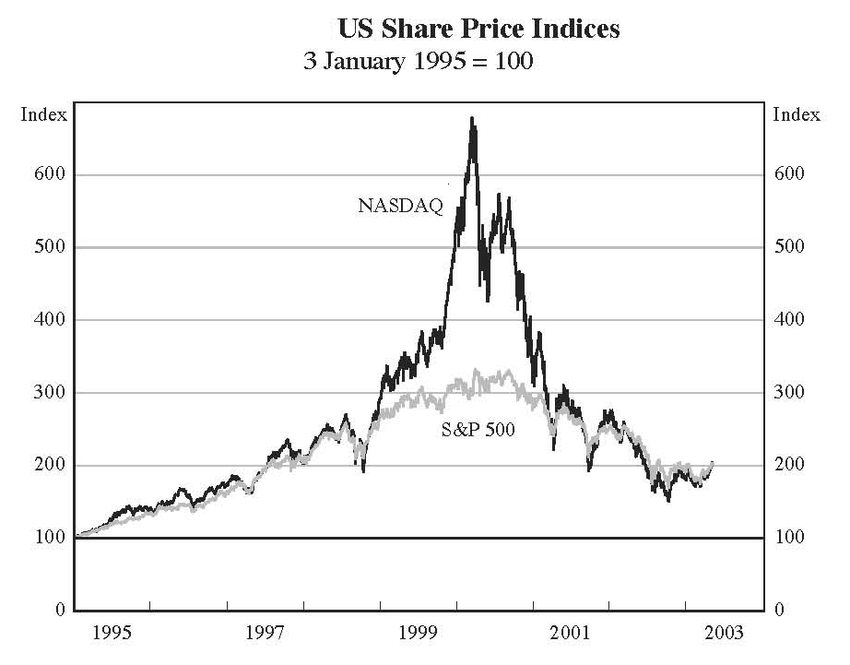
\includegraphics[scale=0.5]{Nasdaq}
\caption{Nasdaq Share prices during the DotCom Bubble}
\autocite{Chisu2018}
\end{figure}

\section{Bitcoin} \bigbreak

Bitcoin is widely considered as the original cryptocurrency and is the most well-known. Although there were earlier attempts at creating digital currencies using cryptography, Bitcoin is the only one that has survived, and is still thriving today. In 2008 the Bitcoin whitepaper titled ‘ Bitcoin: A Peer-to-Peer Electronic Cash System ‘ was sent out a cryptography mailing list. The paper was distributed under the pseudonym of Satoshi Nakamoto, whose real identity is still a mystery to this day. One year later in 2009, the Bitcoin software became publicly available and the network started handling transactions. \autocite{Marr2017} \bigbreak

Bitcoin allows for users to transact with each other using bitcoins, without the need of a third party such as a bank. It achieves this by implementing a public, permanent, continually available and decentralized ledger. The transactions are verified using cryptography, as a chain of digital signatures, known as a blockchain. The network is supported by using proof-of-work, where transactions are validated using computer processing power.\autocite{Nakamoto2008} People who contribute to the network by downloading the Bitcoin software and providing their computing power, are known as miners.  \autocite{Baker2023} \bigbreak

Miners who successfully validate transactions on the network through their own computing power, are rewarded by a predetermined amount of bitcoins. This reward system halves every 4 years, meaning the miners get reduced rewards per processed transaction.{Baker2023} Currently there are 19 million bitcoins in circulation,in 2140 the last Bitcoin will be mined and the proposed limit of 21 million bitcoin should be reached. When that happens, it is presumed that miners will be rewarded by  the transaction fees of users. \autocite{Lewis2018b} \bigbreak
\begin{figure} [h]
    \centering
    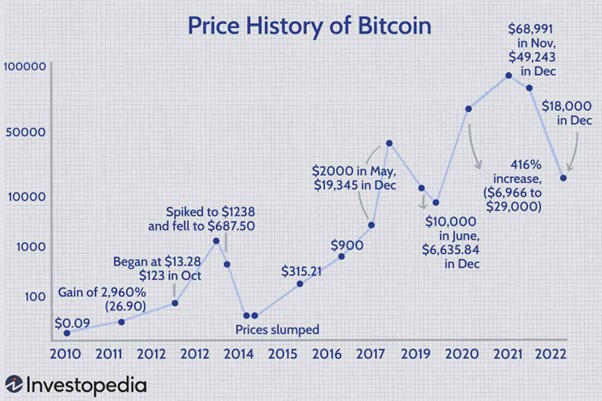
\includegraphics[scale=0.7]{Bitcoin_price}
    \caption{Price History of Bitcoin}
    \autocite{Edwards2023}
\end{figure}
\bigbreak
The price of a single Bitcoin has fluctuated heavily throughout it’s short history. When the technology was first introduced it had a price of zero, during the following years it experienced several boom and bust cycles. In November of 2021 the price of a single bitcoin peaked at around \$69,000 dollar and a total market capitalization of 1,27 trillion dollars. As of writing this paper, the price of a single Bitcoin sits at around \$29 000 dollars. \autocite{Edwards2023} \bigbreak

\section{Dogecoin} \bigbreak

Dogecoin was originally created as a joke in December 2013 by two software engineers, Jackson Palmer and Billy Markus. As the cryptocurrency market was attracting attention for the first time, the duo decided to create a currency based on the dog from the ‘doge’ meme, which was popular at the time. Although it was never meant to be anything other than a parody of other existing cryptocurrencies,the cryptocurrency became an immediate success within online communities. The official dogecoin.com site was visited over a million times within the first month of launching. \autocite{Kay2021} \bigbreak

The technology behind the currency was largely copied from the source code of an already existing cryptocurrency named Litecoin, which in turn was copied from Bitcoin. However, unlike Bitcoin and Litecoin which both have a limited total supply, Dogecoin has an infinite supply with a stable mining rate\autocite{Frankenfield2022}. This makes Dogecoin a highly inflationary asset with over 5 billion Dogecoins being mined each year \autocite{Nibley2022}. \bigbreak

Despite Dogecoin’s technological limitations, its highly inflationary nature and humorous origin, the currency has become one of the major players within the cryptocurrency market. This is mainly due to the strong community behind the project, stemming from the social media website Reddit. In 2014 users of the website utilized the currency in order to tip other users, as a way of repaying them for sharing good ideas or solving a problem \autocite{Frankenfield2022}. \bigbreak

This niche of online supporters steadily grew in the following years, but it wasn’t until 2021 that the currency gained widespread attention. Several high profile celebrities like Elon Musk, Mark Cuban and Snoop Dogg started to publicly support the project, causing the price to surge heavily\autocite{Kay2021}. In May of 2021 the value of a single dogecoin hit \$0.50, a rise of more than 20 000\% in a single year. On the 8th of May 2021 the value peaked at \$0.73 with a total market capitalization of more than 88 billion dollars. Currently the price of a single Dogecoin is \$0,09, a 87\% decrease from it’s all time high value, once again displaying the significant volatility of cryptocurrencies \autocite{Coingecko2023}. \bigbreak

\section{Solana}\bigbreak

Solana is a relatively new cryptocurrency which has become increasingly popular over the last couple of years. The initial whitepaper was first published in 2017 by Anatoly Yakovenko, and the actual network was launched in March of 2020. Solana’s main purpose is to offer a faster and more scalable alternative to more traditional blockchains, achieving this by using innovative technologies and a novel consensus algorithm. \autocite{Picardo2022} \bigbreak

Unlike more traditional blockchains which use the proof of work consensus model, Solana operates using a combination of Proof of History (PoH) and Proof of Stake (PoS)\autocite{Picardo2022}. This means that the network doesn’t have miners, instead users can stake coins with validators which validate the transactions. Staking rewards participants for locking up their personal coins with a validator, receiving the transaction fees of the network in the native currency. Proof of Stake is seen as a more innovative, and has a lower barrier to entry when compared to Proof of Work. Users don’t need to set up their own mining equipment and the energy efficiency is much higher. \autocite{Frankenfield2023} \bigbreak


The aforementioned technological advancements made Solana stand out from its competitors. Rival networks like Ethereum can process around 15 transactions per second, while the Solana network processes more than 50,000 transactions per second. In addition, the transactions fees are significantly lower, with the average transaction fee being around \$0.001 on Solana compared to Ethereum’s \$1.68 \autocite{Picardo2022} \bigbreak


All of these factors contributed to Solana’s success, making it one of the most popular networks in a short period of time\autocite{Jafar2021}. This was also reflected in the value of the token, which rose from 2\$ dollars in November 2020 to it’s peak of \$259 dollars a year later, with a total market cap of 75 billion dollars. A total increase of 12850\%, one of the biggest ever recorded within the cryptocurrency market. \autocite{Coingecko2023a} \bigbreak


\section{State of the art}\bigbreak

The cryptocurrency market has seen an incredible growth over the last 14 years. From only being discussed within niche online forums, to having millions of users worldwide. All the relevant metrics show that the cryptocurrency market has grown immensly and is here to stay for the foreseeable future. As of 2023 it is estimated there are 420 million cryptocurrency users around the world, this is up from 5 million in 2016, a 8000\% + growth rate\autocite{DeBest2023}. During the same period of time, the total market capitalization of all the cryptocurrencies increased from 10 billion dollars to 3 trillion dollars at it’s peak, an 29,900\% increase. \autocite{Coingecko2023b} \bigbreak

But who are the people behind these numbers ? Research show that cryptocurrencies are very popular among younger investors, who are very familiar with the Internet. According to Binance, the biggest worldwide cryptocurrency exchange\autocite{Coinmarketcap2023}, the average age of their userbase is around 34 years old\autocite{Binance2021}. With another study by Forbes discovering that almost half of all American men between ages 18 and 29 have used or invested in cryptocurrencies.\autocite{Delatto2022} \bigbreak 

This new wave of young, tech-savvy investors operate much differently compared to more traditional stock market investors. 80\% of Binance users list online channels as their most important source when it comes to learning about cryptocurrencies and choosing their investments. With social media such as Reddit, Youtube and Twitter being the most popular\autocite{Binance2021}. As cryptocurrencies originated on the Internet, it should be no surprise that most of the related information can be found online. A lot of the established financial institutions and news outlets don’t offer real cryptocurrency investment advice and until recently they avoided the topic. This led to retail investors using social media websites and forums as their main source of information. \autocite{Binance2021} \autocite{Magnusson2022}  \bigbreak

A new term has even been coined which is the ‘Finfluencer’, someone who influences the financial decisions of their followers\autocite{CambridgeWords2021}. Some investors do acknowledge the risk of blindly following social media accounts, but most of them seem to be okay with it, as they regard cryptocurrencies an inherently risky investment.\autocite{Magnusson2022} \bigbreak 
 
Predicting the future price of a specific cryptocurrency is notoriously difficult and it depends on several factors, one of them being market sentiment\autocite{Lewis2018a}. As mentioned earlier, market sentiment refers to how the general public behaves or feels towards a certain asset\autocite{Smith2022}. If investors use these online channels to discuss and share their opinions on certain cryptocurrencies, perhaps it would be possible to analyze these discussions and get an insight into the general sentiment surrounding a certain currency. \bigbreak 

Studies have shown that social media activity can be correlated with an increase in price and trading volume of the mentioned cryptocurrencies.\autocite{Mai2018} In 2021 Elon Musk famously supported both the Dogecoin and Bitcoin cryptocurrencies. After changing his twitter bio to \#Bitcoin, there was an abnormal return of 18,99\% in the next four hours. When he simply tweeted ‘Doge’, the currency experienced an abnormal return of 17.31\% \autocite{Ante2022}. Lennart Ante, the Co-Founder of the Blockchain Research Lab, called this phenomenon the ‘Musk Effect’.\autocite{Ante2022} \bigbreak

\begin{figure} [h]
    \centering
    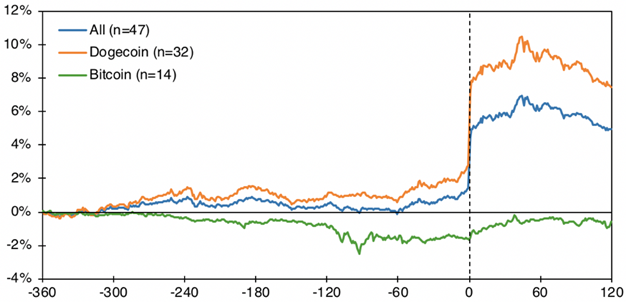
\includegraphics[scale=0.7]{MuskEffect}
    \caption{Effect of Elon Musks tweets on selected Cryptocurrencies}
    \autocite{Ante2022}
\end{figure}


But it is not only Elon Musk’s activity on social media which can influence short term price movements. Other researchers have found that an increase in positive forums posts can predict a rise in trading volume and Bitcoin price in the following days. While the inverse is also true, when negative forums posts are released, the Bitcoin price generally drops during the next couple of days.\autocite{Mai2018} \bigbreak

These previous results lay the foundation of our current research, which is to analyze if there are is a relationship between the sentiment of Tweets and a currencies price action and trading volume. As previous research has shown, social media can have an impact on the market. If we can properly analyze the market sentiment of tweets and find a correlation, it might be a useful addition to the already known effects of social media and it’s relationship with cryptocurrencies. \autocite{Coingecko2023a} \bigbreak  

\textcite{Knuth1998} schreef een van de standaardwerken over sorteer- en zoekalgoritmen. Experten zijn het erover eens dat cloud computing een interessante opportuniteit vormen, zowel voor gebruikers als voor dienstverleners op vlak van informatietechnologie~\autocite{Creeger2009}.


